\subsection{Model 2: learning reward probability from experienced perceptual decisions}

\subsubsection{Model description}

Let stimulus be represented by $x \in \mathbb{R}$, and the corresponding stimulus category $c \in \{0,1\} = H(x-b)$, where $b$ is an unknown category boundary and $H(z)$ is the Heaviside function.

Let the percept be $\hat{x} = x + \epsilon$, where $\epsilon$ is a Gaussian noise term.
The subject must on every trial make a choice $a \in \{0,1\}$ based on $\hat{x}$.
Assuming no catch trials, a trial is rewarded whenever choice $a$ matches stimulus category $c$.
Thus, in order to maximize rewards subjects must be able to estimate category $c$ from knowledge of $\hat{x}$.

Just as in a logistic regression \cite[Section 4.3.2]{bishop2006pattern}, the posterior probability of stimulus category $c$ can be written as a logistic sigmoid $g(z)$ acting on a linear function of the percept $\hat{x}$:
\begin{align}
g(z) &= \frac{1}{1+\exp(-z)} \\
P(c = 1 \mid \hat{x}) &= g(m(\hat{x}-\hat{b})) \label{eq:Pcgperc} \\
P(c = 0 \mid \hat{x}) &= 1 - g(m(\hat{x}-\hat{b}))
\end{align}
with $m, \hat{b} \in \mathbb{R}^+$.
%Thus, a greedy decision rule can be defined as $a = H(\hat{x}-\hat{b})$, where the decision boundary $\hat{b}$ must be learned to approximate the true category boundary $b$.

For a data set with $N$ trials, the likelihood of observed stimulus category as a function of parameters  $m, \hat{b}$ can be written as 
\begin{equation}
    P(\mathbf{c} \mid m, \hat{b}) = \prod_{n=1}^N g(m(\hat{x}_n-\hat{b}))^{c_n} \left(1-g(m(\hat{x}_n-\hat{b}))\right)^{(1-c_n)}
\end{equation}

Parameters can then be learned by minimizing the negative log likelihood
\begin{equation}
    L = - \sum_{n=1}^N
    {c_n} \log g(m(\hat{x}_n-\hat{b})) + 
    {(1-c_n)} \log \left(1-g(m(\hat{x}_n-\hat{b}))\right)
\end{equation}

A subject performing the task could minimize $L$ on the flight by stochastic gradient descent, that is, by computing on each trial the gradient $ \nabla L = \left[\frac{\partial L}{\partial m}, \frac{\partial L}{\partial \hat{b}} \right]^T $ and using it to update its parameter estimates.

Specifically, for trial $n$ and $z_n = m(\hat{x}_n-\hat{b})$, it is useful to establish
\begin{align}
     \frac{\partial L}{\partial z_n} &= \frac{\partial}{\partial z_n}\left[ -{c_n} \log g(z_n) -
    {(1-c_n)} \log \left(1-g(z_n)\right) \right] \nonumber \\
    %        &=  (-c_n) g(z_n)^{-1} g(z_n) \left(1-g(z_n)\right) \nonumber  \\
    %        &- (1-c_n) (-1)  \left(1-g(z_n)\right)^{-1} g(z_n) \left(1-g(z_n)\right) \nonumber \\
    %        &=  (-c_n) \left(1-g(z_n)\right) + (1-c_n) g(z_n)   \nonumber \\
    %        &=  (-c_n) + c_n g(z_n) + g(z_n) -c_n g(z_n)   \nonumber \\
    &=   g(z_n) -c_n   \label{eq:dLdz} \\
    \frac{\partial z_n}{\partial \hat{b}} &= -m \\
    \frac{\partial z_n}{\partial m} &= \hat{x} - 
    \hat{b}
\end{align}

from what it follows by the chain rule that

\begin{align}
    \nabla L &=
    \begin{bmatrix}
    (\hat{x}-\hat{b}) (g(z_n) - c_n)   \\
    m (c_n - g(z_n))
    \end{bmatrix}
\end{align}

Parameter updating would then proceed according to
\begin{align}
    m_{n+1} &= m_{n} - \eta (\hat{x}-\hat{b}) (g(z_n) - c_n) \\
    \hat{b}_{n+1} &= \hat{b}_{n} - \eta m (c_n - g(z_n)) \label{eq:update_b}
\end{align}
where $\eta$ is a step size (learning rate) parameter.

\subsubsection{Simulation}
With parameters $\hat{b}, m$ initialized to $0$, the model was run for $10^5$ trials with different levels of sensory noise $\epsilon$.
Decision boundary quickly converged to its true value $0.5$, and oscillated around it throughout learning.
The slope parameter $m$ consistently converged, albeit to different values depending on levels of sensory noise (figure \ref{fig:mod3}, left column).

\begin{figure}[h!]
    \centering
    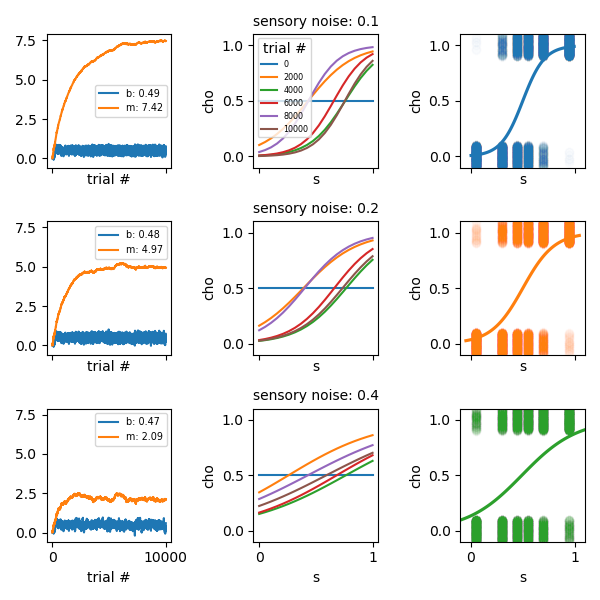
\includegraphics[width=.8\linewidth]{dual2afc/myplot3.png}
    \caption{Model 2, at different levels of sensory noise (rows). \\
    (left) Learning of decision boundary $\hat{b}$ and slope $m$ is stable. \\
    (center) Learned sigmoid at different stages of learning. \\
    (right) Psychometric curve at the end of learning.}
    \label{fig:mod3}
\end{figure}

An agent whose only concern is to get the perceptual decision right (ie. no time investment decision), has only to learn the decision boundary $\hat{b}$, and could thus set $m$ to any constant value in $\mathbb{R}_+$, say $m=1$ for convenience.
%The learning equation \ref{eq:update_b} could then drop the $m$ term, and could probably be expressed in terms of reward rather than category $c$.
Notice that the magnitude of the update of $\hat{b}$ (equation \ref{eq:update_b}) still depends on the distance between percept and boundary (since  $z_n = m(\hat{x}_n-\hat{b})$).

However, if the agent is also learning a time investment decision, it will probably be required to estimate $P(c \mid \hat{x})$ (equation \ref{eq:Pcgperc}), which depends on $m$.
In fact, psychometric curves observed under different noise levels were captured by different values of $m$  (figure \ref{fig:mod3}).
%given that $H(g(m(\hat{x}-\hat{b})))$ does not depend on $m$,